%uiuc-es-figure.tex

\documentclass[a4]{article}

\usepackage{varwidth}
\usepackage{tabularx}
\usepackage{tikz}
\usepackage{amsmath}
\usepackage{graphicx}
\usetikzlibrary{shapes.geometric, arrows, chains}
\usetikzlibrary[calc]


\tikzstyle{load} = [rectangle, minimum width=1cm, minimum height=1cm, text centered, draw=black, execute at begin node = \begin{varwidth}{5cm}, execute at end node=\end{varwidth}]
\tikzstyle{supply} = [diamond, minimum width=2cm, minimum height=1cm, text centered, draw=black, fill=orange!30, execute at begin node = \begin{varwidth}{1.5cm}, execute at end node=\end{varwidth}]
\tikzstyle{decision} = [circle, minimum width=1cm, minimum height=1cm, text centered, draw=black, execute at begin node = \begin{varwidth}{1.5cm}, execute at end node=\end{varwidth}]
\tikzstyle{arrow} = [thick,->,>=stealth]
\tikzstyle{extra} = [rectangle, minimum width=1cm, minimum height=1cm, text centered, draw=black, fill=green!30, execute at begin node = \begin{varwidth}{3cm}, execute at end node=\end{varwidth}]
\tikzstyle{import} = [rectangle, minimum width=1cm, minimum height=1cm, text centered, draw=black, fill=red!30, execute at begin node = \begin{varwidth}{3cm}, execute at end node=\end{varwidth}]
\tikzstyle{flexible} = [diamond, minimum width=1cm, minimum height=1cm, text centered, draw=black, fill=blue!30, execute at begin node = \begin{varwidth}{3cm}, execute at end node=\end{varwidth}]


\begin{document}
	

	\begin{figure}
		\caption{\textbf{UIUC Embedded Grid System Flowchart}}
		\centering
		\vspace{2cm}
		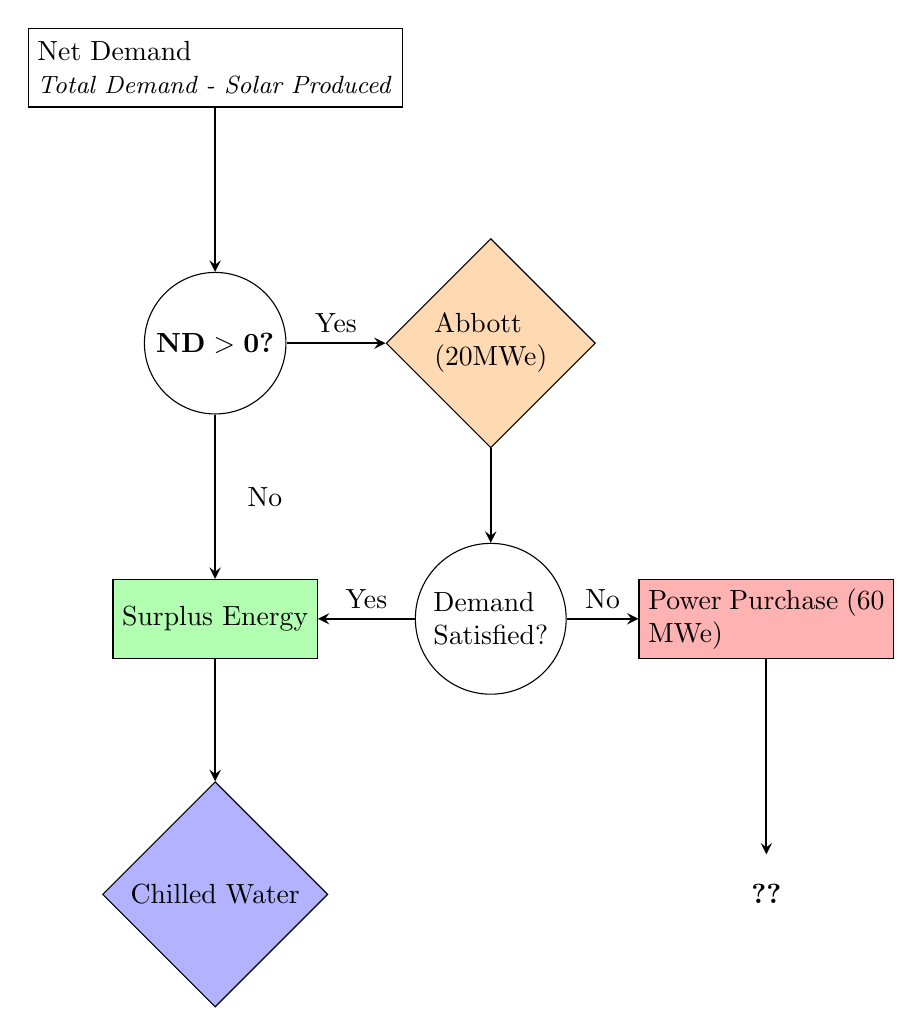
\begin{tikzpicture}[node distance = 3.5cm, auto]
			\node (demand) [load] {Net Demand\\\small{\textit{Total Demand - Solar Produced}}};
			\node (ND) [decision, below of = demand] {\textbf{ND $>$ 0?}};
			\node (abbott) [supply, right of = ND] {Abbott (20MWe)};
			\node (isfull) [decision, below of = abbott] {Demand Satisfied?};
			\node (surplus) [extra, left of = isfull] {Surplus Energy};
			\node (purchase) [import, right of = isfull] {Power Purchase (60 MWe)};
			\node (chilledwater) [flexible, below of = surplus] {Chilled Water};

			\node (d1) [load, draw=none, below of = purchase] {\textbf{??}};

			\draw [arrow] (demand) -- (ND);
			\draw [arrow] (ND) -- node [text width = 1cm, midway, align=center] {No} (surplus);
			\draw [arrow] (ND) -- node [text width = 1cm, midway, above, align=center] {Yes} (abbott);
			\draw [arrow] (abbott) -- (isfull);
			\draw [arrow] (isfull) -- node [text width = 1cm, midway, above, align=center] {Yes} (surplus);
			\draw [arrow] (isfull) -- node [text width = 2cm, midway, above, align=center] { No } (purchase);
			\draw [arrow] (surplus) -- (chilledwater);
			\draw [arrow] (purchase) -- (d1);
		\end{tikzpicture}
	\end{figure}


\end{document}